\documentclass{article}
\usepackage[utf8]{inputenc}
\usepackage{graphicx}
\usepackage{here}
\usepackage{amsmath}
\usepackage{amsfonts}

\title{Notes de cours\\OPT6 : Apprentissage avancé}
\author{Adrien Pavao}
\date{Novembre 2017}

\begin{document}

\maketitle

%\tableofcontents

\section{Introduction}

Apprentissage avancé. Le domaine de l'apprentissage automatique évolue vite.

\subsection{Quelques notions}
\begin{itemize}
\item Vladimir Vapnik a posé les bases théoriques de l'apprentissage statistique\footnote{https://en.wikipedia.org/wiki/Statistical\_learning\_theory}.
\item Apprentissage PAC : Probably Approximately Correct\footnote{https://en.wikipedia.org/wiki/Probably\_approximately\_correct\_learning}.
\item \textbf{No-free-lunch theorem :} Il n'existe pas de méthode d'apprentissage qui soit meilleure qui les autres. Même performance que l'aléatoire sur l'ensemble des problèmes possibles. Si une méthode est efficace sur un problème elle sera mauvaise sur un autre. L'intégrale sur tous les problèmes est toujours la même, quelque soit la méthode. Idem pour les mesures (de distance par exemple). Les méthodes sont adaptées à des \textbf{classes} de problèmes. \textbf{Tous les algorithmes inductifs se valent.}
\item \textbf{Adversarial learning :} L'intersection entre le machine learning et la sécurité informatique.
\item Ordre $L_0$, $L_1$ $\rightarrow$ à chercher. 
\item \textbf{Distance de Manhattan :} La distance entre deux points lorsque les déplacements sont faits selon un réseau ou un quadrillage. 

\begin{figure}[H]
    \begin{center} 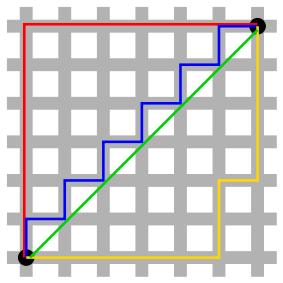
\includegraphics[scale=0.5]{manhattan.png} \end{center}
     \caption{Distance de Manhattan (chemins rouge, jaune et bleu) contre distance euclidienne en vert.}
\end{figure}

Le nom de cette distance fait sans doute référence à l'architecture en quadrillage du quartier de Manhattan, à New York.

\item Référence d'un livre intéressant : \textit{Hofstadter - "Godel, Escher, Bach".}
\item \textbf{Complexité de Kolmogorov :} Une fonction permettant de quantifier la taille du plus petit algorithme nécessaire pour engendrer un nombre ou une suite quelconque de caractères. Cette quantité peut être vue comme une évaluation d'une forme de complexité de cette suite de caractères.
\item Effets de séquences : Une séquence d'information influe sur le résultat de l'induction (à préciser).
\item L'algorithme d'apprentissage du perceptron converge si les données sont linéairement séparables. Cette convergence est en nombre fini d'étapes et ce nombre est indépendant du nombres d'exemples, de la distribution des exemples, et quasiment pas de la dimension de l'espace d'entrée. Il dépend de la marge de séparation des nuages de points et du diamètre de la boule (à préciser).
\item \textbf{L'espace des versions :} Toutes les hypothèses correctes (qui ne font pas d'erreurs) d'après les données d'apprentissage.
\end{itemize}

\section{Induction}

On déduit à partir d'un échantillon.

\begin{enumerate}
\item Espace d'hypothèse H.
\item Critere inductif $ S \times h \in H \rightarrow $ Score $\in \mathbb{R}$. Par exemple minimiser le taux d'erreur.
\item Methode d'exploration de H.
\end{enumerate}

On ne dispose pas de théorie bien établie de l'induction (exemple Fibonacci).

\subsection{Différents types d'apprentissage}
\begin{itemize}
\item \textbf{Descriptif :} Non supervisé. On cherche des régularités dans les données. On ne souhaite pas extrapoler, on ne s'interesse qu'à l'échantillon de données dont on dispose. La "matière noire" de l'apprentissage.
\item \textbf{Prédictif :} Supervisé. L'échantillon de données sert à apprendre une hypothèse sur les données pour prédire ensuite sur de nouvelles données. On cherche des corrélations entre les données.
\item \textbf{Prescriptif :} On cherche des \textbf{causalités}. Il s'agit d'une tâche difficile.
\end{itemize}

Les frontières entre ces types d'apprentissage peuvent être floues, on peut par exemple commencer par une description des données pour les comprendre avant de faire un modèle prédictif.

\subsection{Différentes méthodes d'apprentissage}

\begin{itemize}

\item Méthodes d'ensemble (clustering).

\item Supervisé.

\item L'induction :
    \begin{itemize}
    \item Apprentissage semi supervisé 
    \item Apprentissage de modèles parcimonieux (peu de paramètres).
    \end{itemize}

\item Apprentissage en ligne (online learning) : Les données arrivent en cours de route.

\item \textbf{Apprentissage par transfert :} Cela vise à transférer des connaissances d'une ou plusieurs tâches sources vers une ou plusieurs tâches cibles. On peut le voir comme la capacité d’un système à reconnaître et appliquer des connaissances et des compétences, apprises à partir de tâches antérieures, sur de nouvelles tâches ou domaines partageant des similitudes.

\end{itemize}

\subsection{Types de biais}

L'induction necessite d'être biaisé, d'avoir une preference pour certaines hypothèses, de ne pas connaitre toutes les fonctions possibles. Un biais classique et très humain est la préférence des hypothèses les plus simples (rasoir d'Ockham).

\begin{itemize}
\item \textbf{Biais de représentation (déclaratif) :} On ne peut représenter qu'un petit nombre de fonctions possibles. Le langage dans lequel on exprime le problème ne me permet pas de tout représenter.
\item \textbf{Biais de recherche (procédural) :} La procédure de recherche avantage certaines hypothèses. Par exemple on reste proche de notre point initial de recherche dans l'espace des fonctions possibles.
\end{itemize}

Souvent un peu des deux.

\subsection{Risques}

On distingue deux types de risques :

\begin{itemize}
\item \textbf{Risque réel} (ce que l'on veut minimiser). La performance à venir si j'utilise l'hypothèse h. Cela prend la forme d'une espérance de coût d'usage de h. Le risque réel (loss function) : 
\[ R(h) = \displaystyle \int_X^Y l(h(x), y) p(x, y) \mathrm{d}x \mathrm{d}y \]

La meilleure hypothèse est $k\star = Argmin R(h)$ avec $h \in H$. En d'autres termes, on cherche l'hypothèse qui minimise le risque réel. $l$ est la métrique d'évaluation et $p$ la loi de probabilité hypothétique ayant générée la distribution des données.
\item \textbf{Risque empirique}. Puisque l'on cherche la loi de probabilité, on ne la connait pas et on ne peut donc pas s'en servir pour calculer le risque, en pratique. On calcul donc le risque empirique : 
\[ \hat{R}(h) = \frac{1}{m} \sum_{i=1}^m l(h(x_i), y_i) \]
C'est donc la moyenne des distances entre les prédictions avec h et les valeurs réelles des données. \^h est l'hypothèse minimisant le risque empirique. 
\end{itemize}

On cherche les liens entre toutes ces notions.

\section{Transduction}

On ne s'interesse qu'à un point. Le nombre de données requises pour tirer une conclusion n'est plus influencé par le nombre de dimension. On parle de \textbf{transductive learning}.
\begin{itemize}
\item Transduction : Cas d'induction limite (une question).
\item Analogie : Cas de transduction limite (un exemple).
\end{itemize}
\end{document}


